\documentclass[t,aspectratio=1610]{beamer}

\usepackage{bxcjkjatype}
\usepackage{listings}
\usepackage{tikz}
\newcounter{row}
\newcounter{col}

\newcommand\setrow[9]{
  \setcounter{col}{1}
  \foreach \n in {#1, #2, #3, #4, #5, #6, #7, #8, #9} {
    \edef\x{\value{col} - 0.5}
    \edef\y{9.5 - \value{row}}
    \node[anchor=center] at (\x, \y) {\n};
    \stepcounter{col}
  }
  \stepcounter{row}
}

\usetheme{default}
\beamertemplatenavigationsymbolsempty\setbeamersize{
    text margin left=0.75cm,
    text margin right=0.75cm
}

% Title
\setbeamerfont{title}{size=\LARGE, 
                      series=\bfseries,
                      family=\rmfamily}
\setbeamercolor{title}{fg=blue!70!black}
\setbeamertemplate{frametitle}{
    \nointerlineskip\;
    \begin{beamercolorbox}[sep=.1ex,
                           wd=\paperwidth,
                           leftskip=0.5cm,
                           rightskip=0pt]{frametitle}
        \usebeamerfont{frametitle}
        \usebeamercolor[fg]{frametitle}
        \\
        \hfill
        \insertfrmetitle\;
        \strut\;
    \end{beamercolorbox}
}
% Alerted text
\setbeamerfont{alerted text}{shape=\itshape,
                             series=\bfseries}
\setbeamercolor{alerted text}{fg=black!90}
% Itemize
\setbeamercolor{itemize item}{fg=black!90}
\setbeamercolor{itemize subitem}{fg=black!90}
\setbeamertemplate{itemize item}[circle]
\setbeamertemplate{itemize subitem}[triangle]
% Blocks
\setbeamercolor{block body example}{fg=black!90,
                                    bg=black!10}
\setbeamercolor{block title example}{fg=white,
                                     bg=blue!30!black!30}
\setbeamertemplate{blocks}[shadow=true]

\newcommand{\sidesplit}[4][0.25]{%
    \centering
    \begin{minipage}{#1\textwidth}
    \resizebox{\textwidth}{!}{#2}
    \end{minipage}
    \hfill
    \begin{minipage}{#1\textwidth}
    \resizebox{\textwidth}{!}{#3}
    \end{minipage}
    \hfill
    \begin{minipage}{#1\textwidth}
    \resizebox{\textwidth}{!}{#4}
    \end{minipage}
}


\title{Courses @ USI (CUSI)}
\subtitle{Mobile \& Wearable Computing}
\author{Bevilacqua Joey \\ Lagrasta Federico \\ Rodolfo Masera Tommaso}
\institute{Universit\`a della Svizzera Italiana\\ Faculty of Informatics\\ \href{http://www.unisi.ch}{www.unisi.ch}}
\date{Nov 4, 2021}

\begin{document}
{
% Slide 1: Title slide
% - Name of app and of group members

%\usebackgroundtemplate{\includegraphics[width=1\paperwidth, height=1\paperheight]{screamc}}
\begin{frame}
\maketitle
\end{frame}
}

{
% Slide 2: Motivation slide
% - What is the problem your app is supposed to solve?
% - Why do you expect it to be useful?
% - What’s wrong with existing solutions (if applicable)

\begin{frame}
\textbf{Motivation} \\

\begin{itemize}
\item CUSI aims to help USI students and staff with organizing and keeping track of their courses and schedules
\pause
\item We expect the app to be USI-ful as it will offer a quick and easy-to-access interface to manage courses with the option to customize it with courses from different master and bachelor programmes
\pause
\item Currently the course schedule is accessible only on the USI website, it is hard to navigate via mobile and it does not allow a customizable schedule comprising courses from multiple programmes
\end{itemize}
\end{frame}
}

{
% Slide 3: Project slide
% - Describe how you plan to implemented your app
\begin{frame}
\textbf{Project} \\

\begin{enumerate}
\item The application will retrieve information for all the available courses and will allow the user to add it to their schedule
\pause
\item The application will then display the added courses via a list or a Gantt diagram
\pause
\item Furthermore, it will use GPS and movement sensors to detect the position of the user and will send push notifications if the user is not in the proximity of the campus where the class is going to take place and the he or she is not moving towards it 
\end{enumerate}
\end{frame}
}

{
% Slide 4: Storyboard slide
% - Add the storyboard of your app
\begin{frame}
\textbf{Storyboard} \\

% \vspace{-0.6em}
\centerline{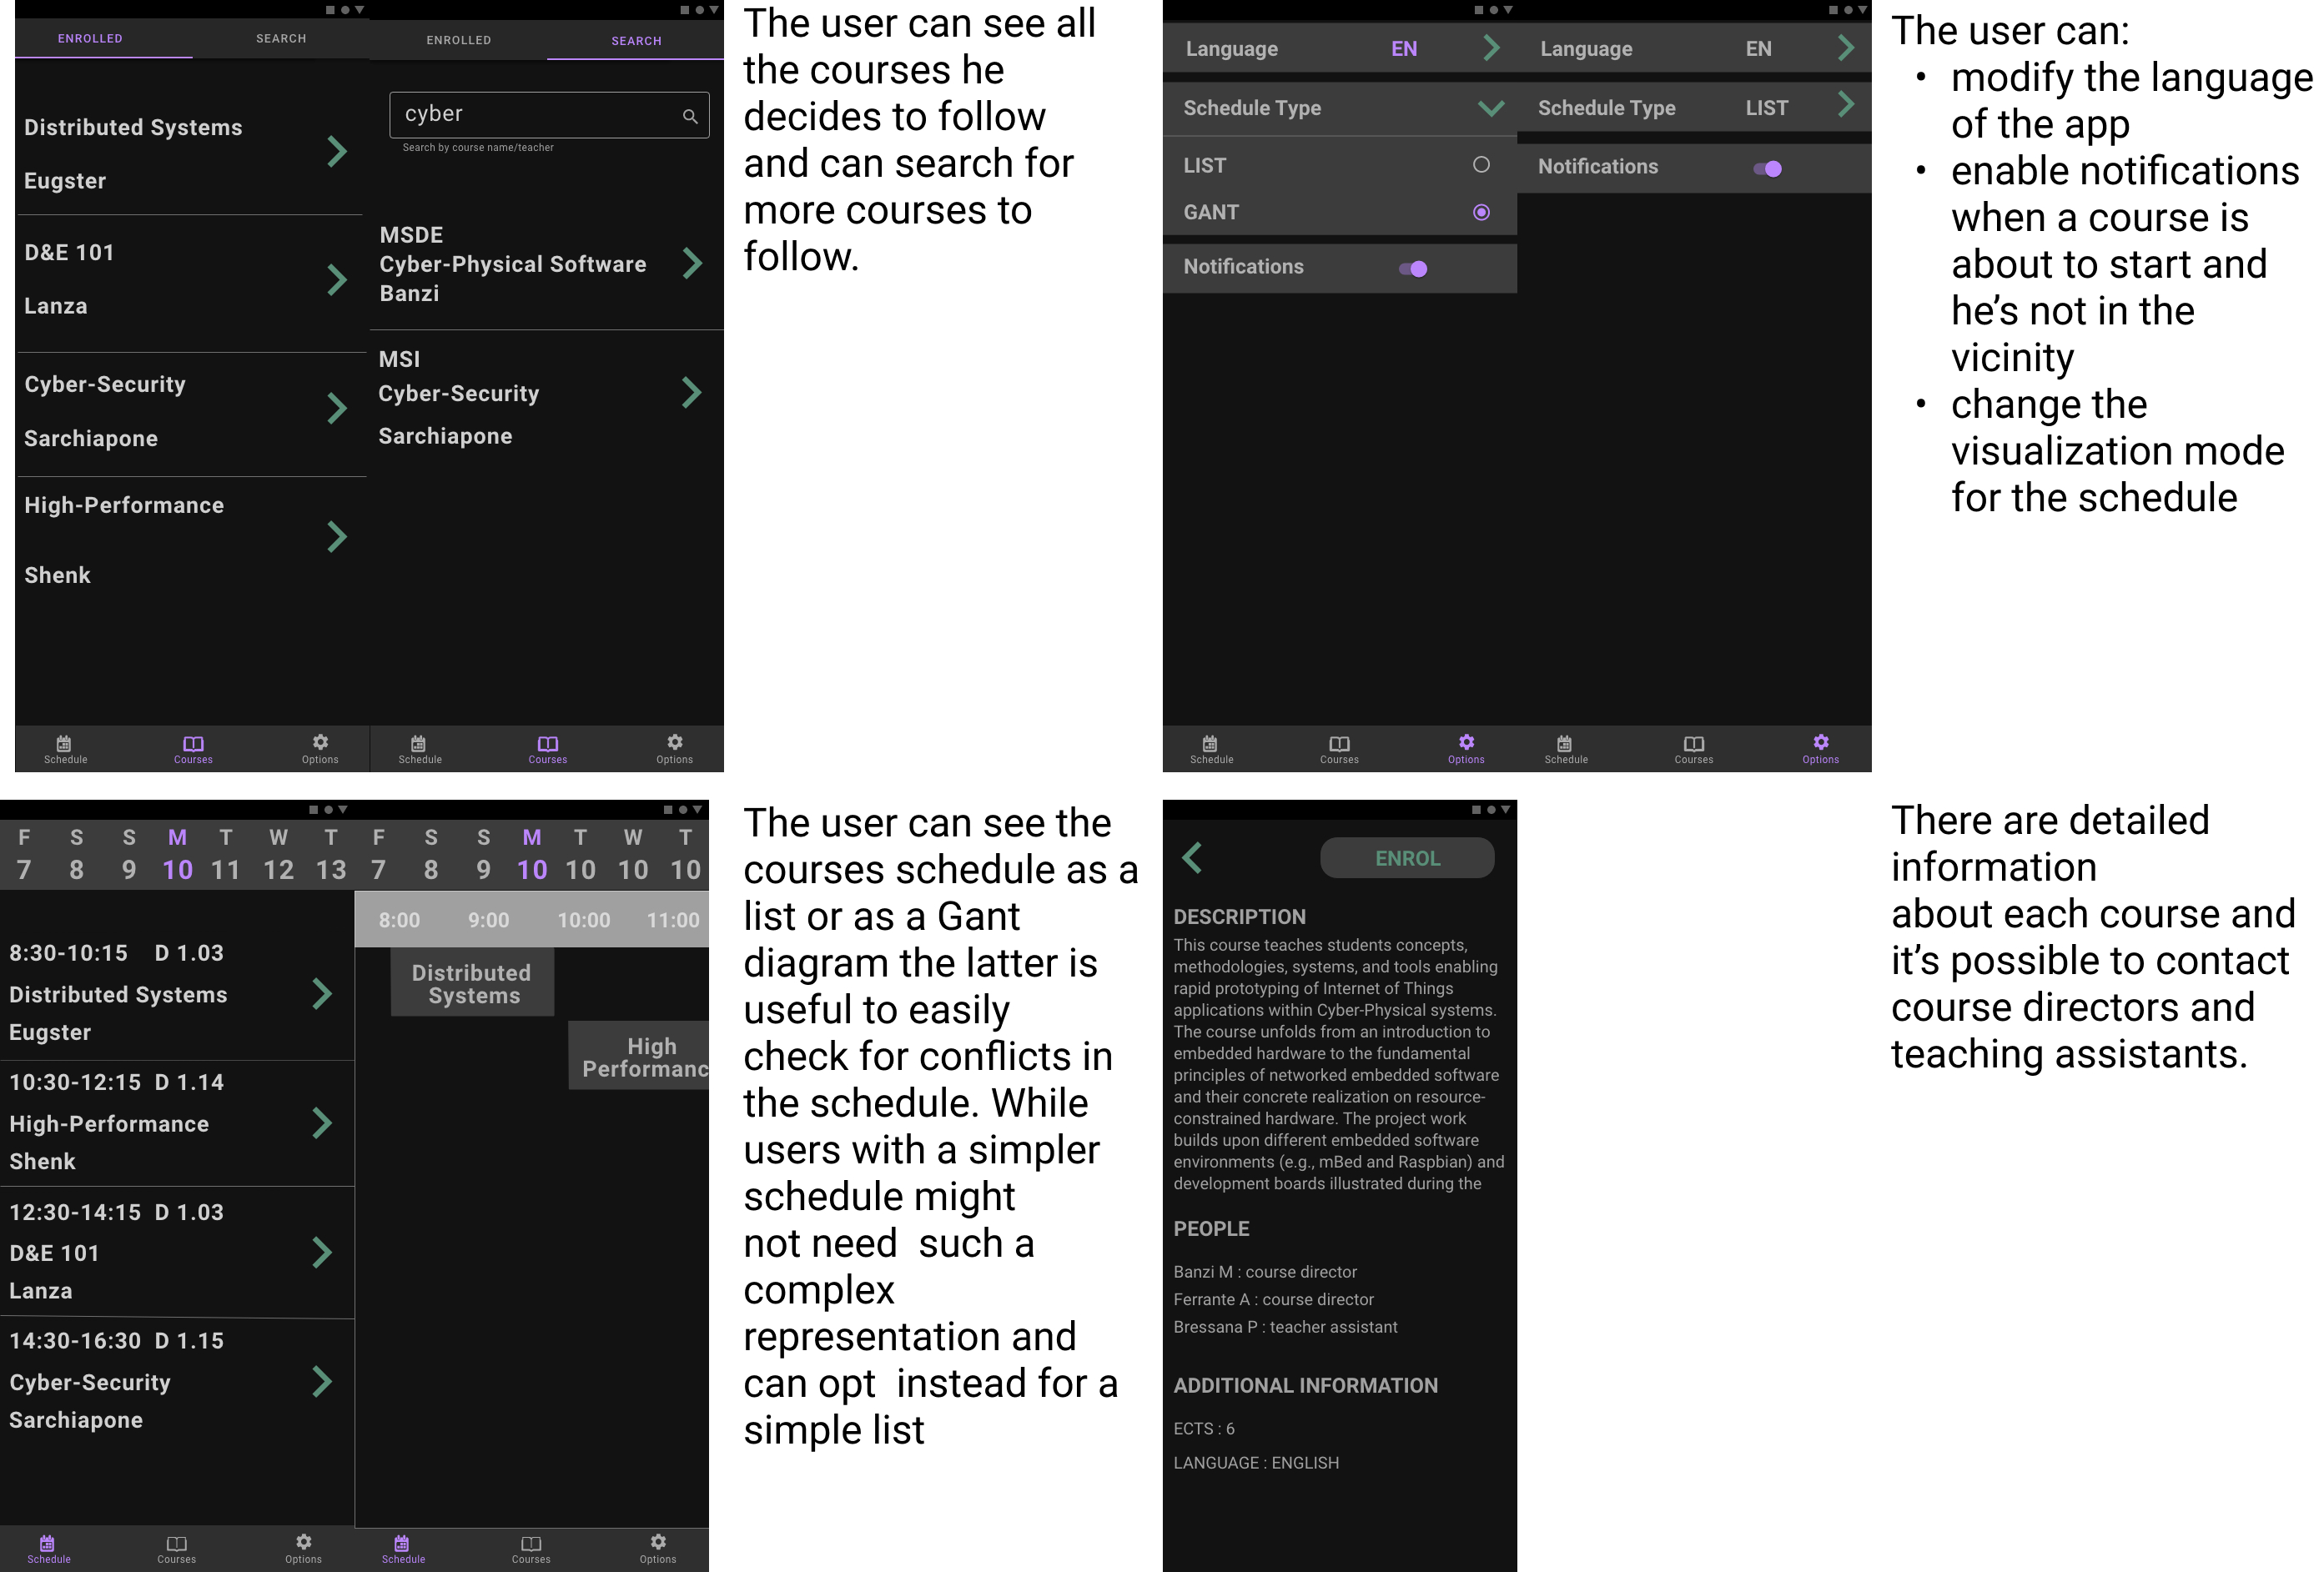
\includegraphics[scale=0.13]{storyboard.jpg}}
\end{frame}
}

{
% Slide 5: Thank you slide
% - Tank you https://youtu.be/usWfJ0EJLB0?t=1047

\begin{frame}
\textbf{Questions} \\
\centerline{
\includegraphics[scale=0.45]{questions}}
\end{frame}
}
\end{document}
